\documentclass[../main.tex]{subfiles}
\subsection{History of the Camping Ban}
In November 2017, the Office of City Auditor released a highly critical report on the effectiveness of Austin's homelessness policy \cite{ordinance_audit}. It disparaged the city ordinances for the barriers created by the excess of arrest warrants issued. It also noted that citations were not effectively connecting unsheltered persons to case management services, as had been promised. The report ultimately recommended either repealing the city ordinances or amending them with less punitive language.

Over the next eight months, the City Council appeared to consider revising the camping ban multiple times, according to a fact sheet produced by councilmember Greg Casar\cite{casar_faq}. In the June 28, 2018 meeting, an agenda item was introduced proposing an amendment to the solicitation ordinance. The item was withdrawn and not discussed during the meeting, but local news outlets began to report that the City Council was on the brink of repealing the anti-homeless city ordinances \cite{austinmonitor}. Enforcement fell sharply (see Section \ref{sec:data} for discussion), and the City Council eventually followed through on what many saw as a foregone conclusion, repealing the solicitation ordinance and amending the sit/lie and camping ordinances to drastically reduce their scope during their June 20, 2019 meeting.

It is important to develop this timeline here before elaborating a model, since it underscores the difficulty in defining a ``high enforcement period'' and ``low enforcement period'' over time. The City Auditor's report noted that the Austin Police Department had already revised their internal guidelines on the sit/lie ordinance in 2017, giving offenders a grace period of 30 minutes before citing and hence precipitating a decline in the number of citations written. Furthermore, there is an intervening period of one year between when the Council effort to repeal the ordinances became public knowledge and when it was enacted. And, even though APD has stopped issuing citations, the Texas Department of Transportation, at the behest of the Governor, still periodically conducts ``sweeps'' that attempt to clear out encampments under state highway overpasses.

Ultimately, I decided to rely on the citation data that I have as a ``good enough'' indicator. I believe there is still a strong structural relationship between \textit{where} citations are issued and the density of unsheltered people in those areas, which I will argue helps provide reduced-form causal evidence.

\subsection{Data on Ordinance Enforcement}
\label{sec:data}
There are two courts in Austin to which citations are referred: the Downtown Austin Community Court (DACC) for citations issued within the downtown area, and the Austin Munipal Court (AMC) for citations issued elsewhere within the city. I obtained all court records for DACC and AMC from January 2015 to December 2019 through the city of Austin's Open Data Portal \cite{open_data_portal}. I then cross-referenced the offense codes listed with data from the \textit{Texas Observer} and filtered out only public camping and no sit/no lie citations. 

Finally, I geocoded the street addresses to latitude, longitude, and census tract. There was a marginal error rate in geocoding—I discarded samples that were geocoded because of an ambiguous address to a location outside of Austin. This constituted much less that 1\% of the sample. 

Figure~\ref{fig:citations_over_time} gives a plot of the citations per month issued from 2015 to 2019. The vertical line in red indicates the date of the City Council meeting of June 28, 2018. The vertical line in green indicates the date of the Council meeting on June 20, 2019.

\begin{figure}
    \begin{center}
        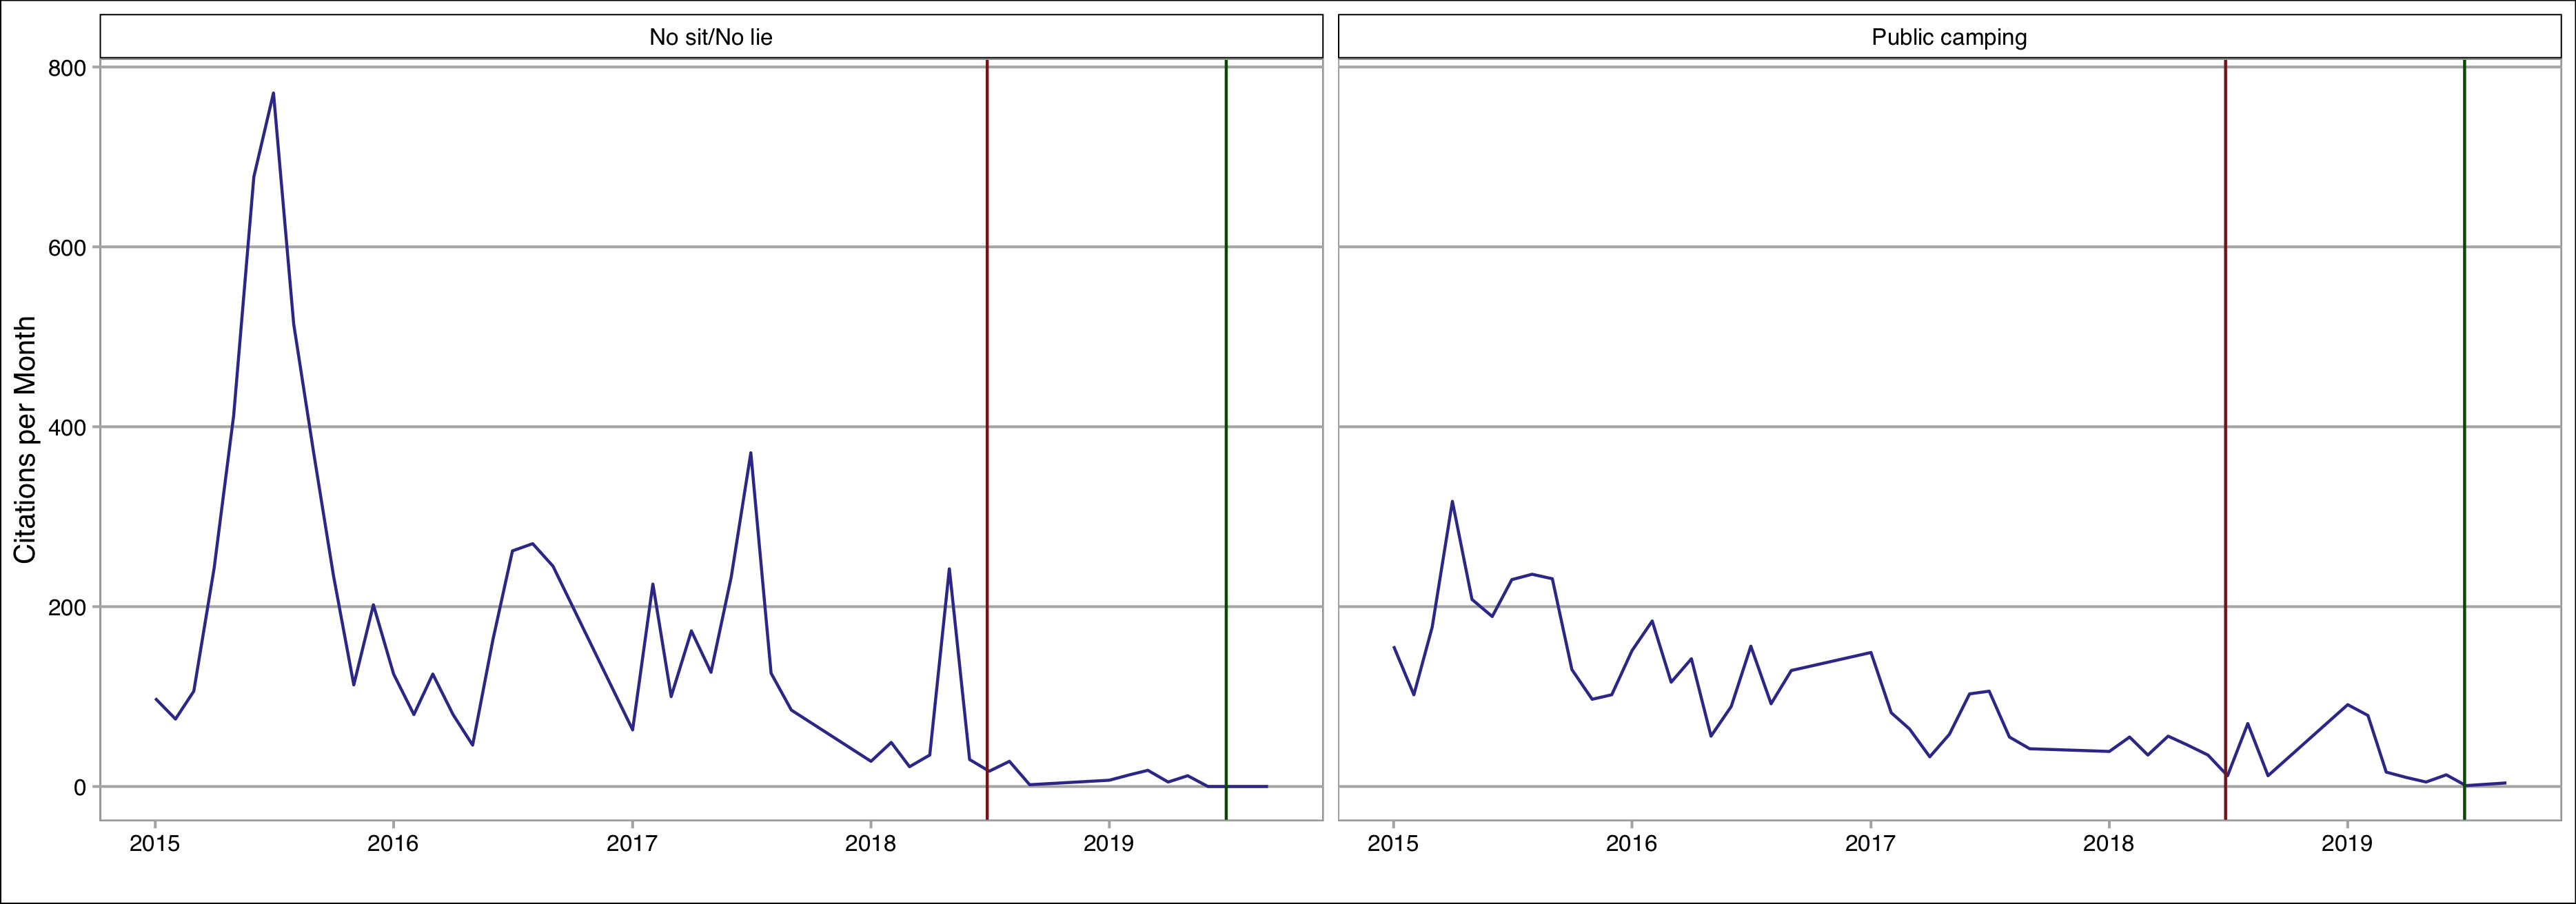
\includegraphics[width=.8\textwidth]{../../figures/citations_over_time.png}
        \caption{Monthly citations for public camping and sit/lie ordinances, 2015–2019. Red line is date of proposed policy change in June 2018, green line is date of implementation in June 2019.}
        \label{fig:citations_over_time}
    \end{center}
\end{figure}

\subsection{Crime Report Data}
I obtained a database of crime reports from the city's Open Data Portal \cite{open_data_portal}. The crime data are subdivided into broad categories of offenses, and I chose to focus on offenses from the ``Theft'' and ``Robbery'' categories. I geocoded all relevant crime reports from 2015 to 2019, again discarding the small proportion of the sample that was mistakenly geocoded outside of Austin.

\subsection{Note on Timeline}

The COVID-19 pandemic created additional complications for both citation and crime data. 